%Preamble
\documentclass[12pt,a4paper]{article}
\usepackage[top=20mm, bottom=20mm, left=20mm, right=20mm]{geometry}
\usepackage[utf8]{inputenc}
\usepackage{fancyhdr} \setlength{\headheight}{15pt}
\usepackage{lastpage}
\usepackage{t1enc}
\usepackage[magyar]{babel}
\usepackage{amsmath}
\usepackage{amssymb,physics}
\usepackage{amsthm}
\usepackage{empheq}
\usepackage{enumitem}
\usepackage{subfiles}
\usepackage{float}
\usepackage{verbatim}
\usepackage{amsmath}
\usepackage{hyperref}
\usepackage{amsmath}
\usepackage{multicol}
\usepackage{blkarray}
\usepackage{tikz}
\usepackage{pgfplots}
\newcommand*\widefbox[1]{\fbox{\hspace{2em}#1\hspace{2em}}}
\pagestyle{fancy}
\def\mx#1{\mathbf{#1}}
\def\vec#1{\underline{\mathbf{#1}}}
\def\m{\; \left[\mathrm{m}\right]}
\def\mili{\; \left[\mathrm{mm}\right]}
\def\deg{\; \left[^{\circ}\right]}
\def\mm{\; \left[\mathrm{m^2}\right]}
\def\i{\left(i\right)}
\def\cosalfa{\cos \alpha^{\i}}
\def\sinalfa{\sin \alpha^{\i}}
\def\cosalfasq{\cos^2 \alpha^{\i}}
\def\sinalfasq{\sin^2 \alpha^{\i}}
\def\Nm{\; \left[\mathrm{\frac{N}{m}}\right]}
\def\kN{\; \left[\mathrm{kN}\right]}
\def\futyi{\cdot 10^{7}}
\def\fos{\; \left[-\right]}
\def\Mpa{\; \left[\mathrm{MPa}\right]}

\lhead{BMEGEMMBXVE, VEM alapjai 1. Szorgalmi HF}
\cfoot{\thepage\ / \pageref{LastPage}}
\rhead{Németh Áron Imre, D1J5ZG}

\begin{document}

\begin{figure}[H]
    \centering
    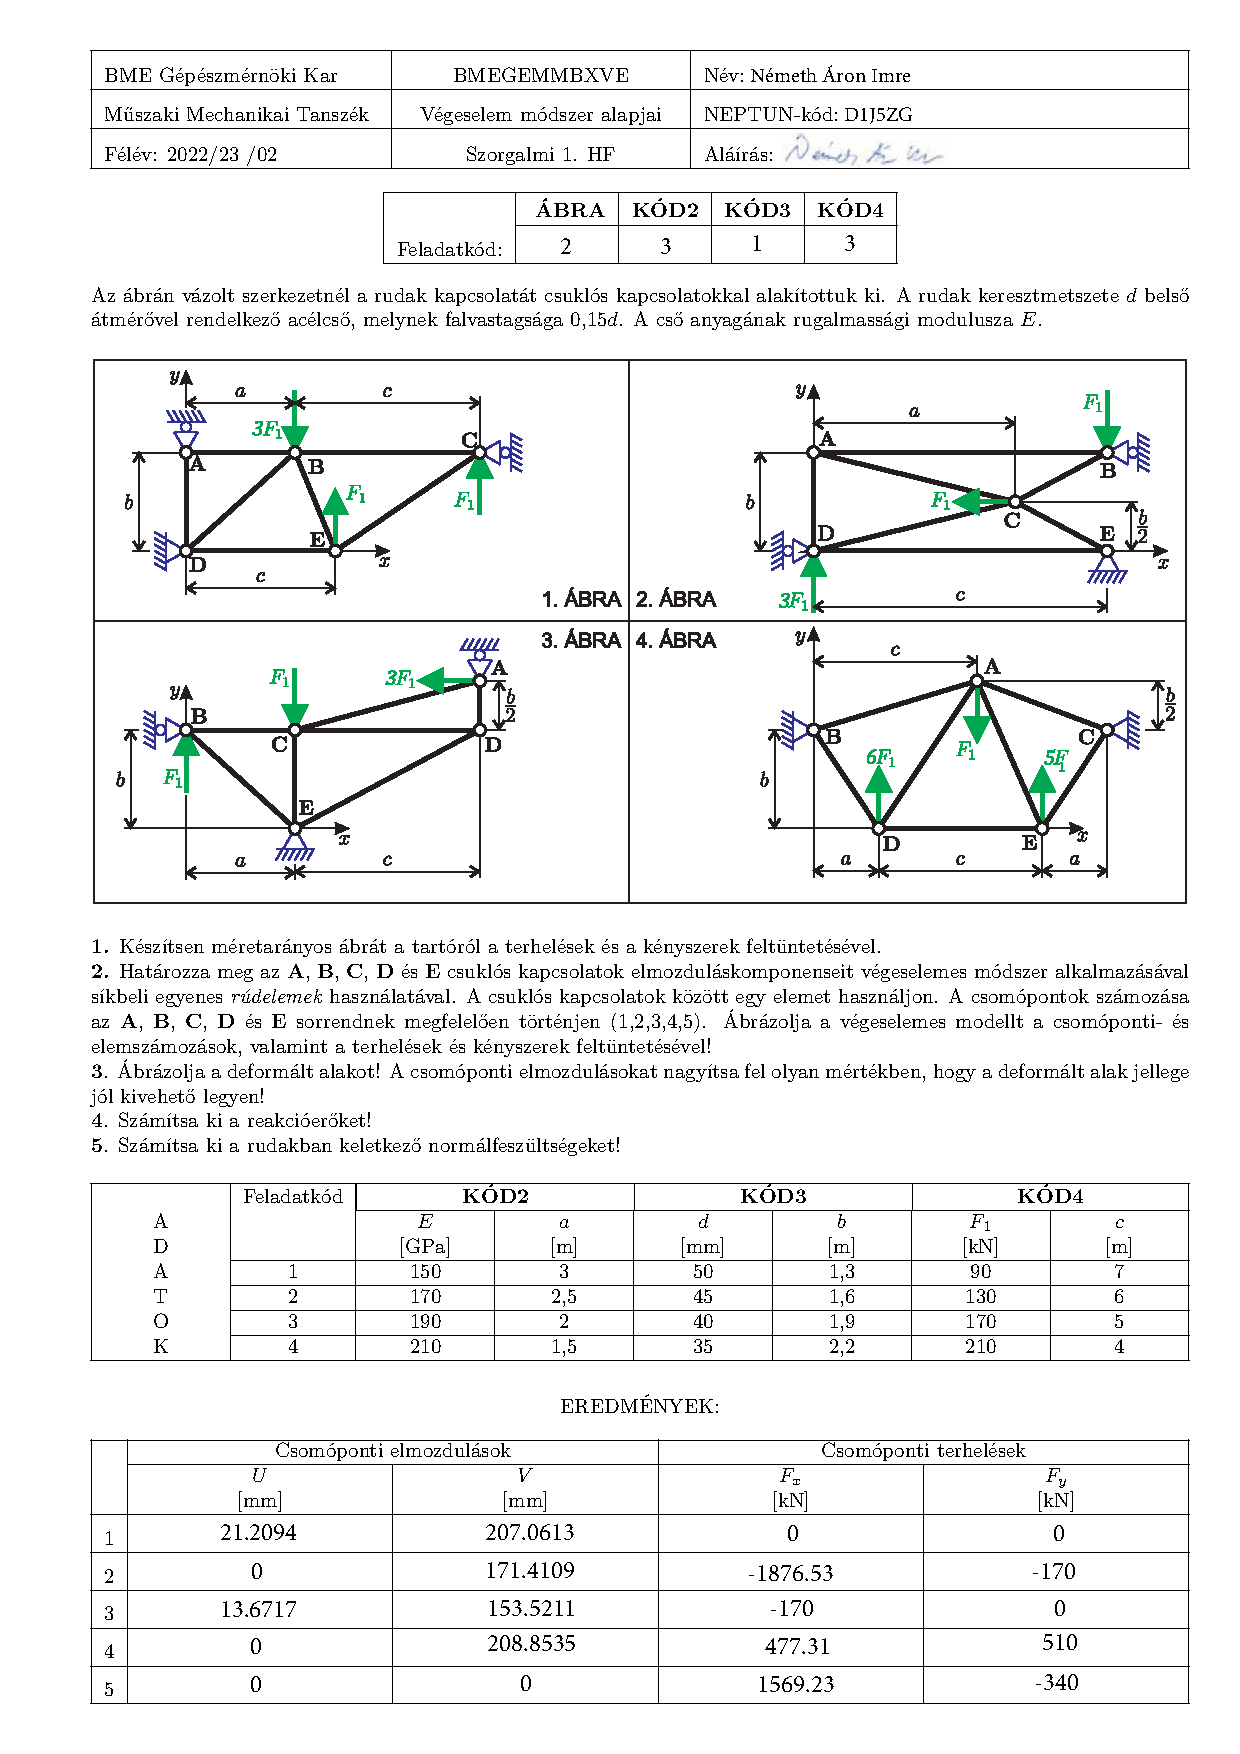
\includegraphics[width=1\textwidth]{szhf1_fedo.pdf}
\end{figure}

\section{A szerkezet méretarányos ábrájának elkészítése}
\subsubsection*{Adatok:}
\begin{multicols}{2}
    \begin{itemize}
        \item $a=2 \m$
        \item $b=1.3 \m$
        \item $c=5 \m$
    \end{itemize}
    \columnbreak
    \begin{itemize}
        \item $d=50 \; \left[\mathrm{mm}\right]$
        \item $E=190 \; \left[\mathrm{GPa}\right]$
        \item $F=170 \; \kN$
    \end{itemize}
\end{multicols}
\subsection{A szerkezet léptékhelyes ábrája}
A szerkezet méretarányos ábrája esetünkben az alábbi módon néz ki:
\begin{figure}[H]
    \centering
    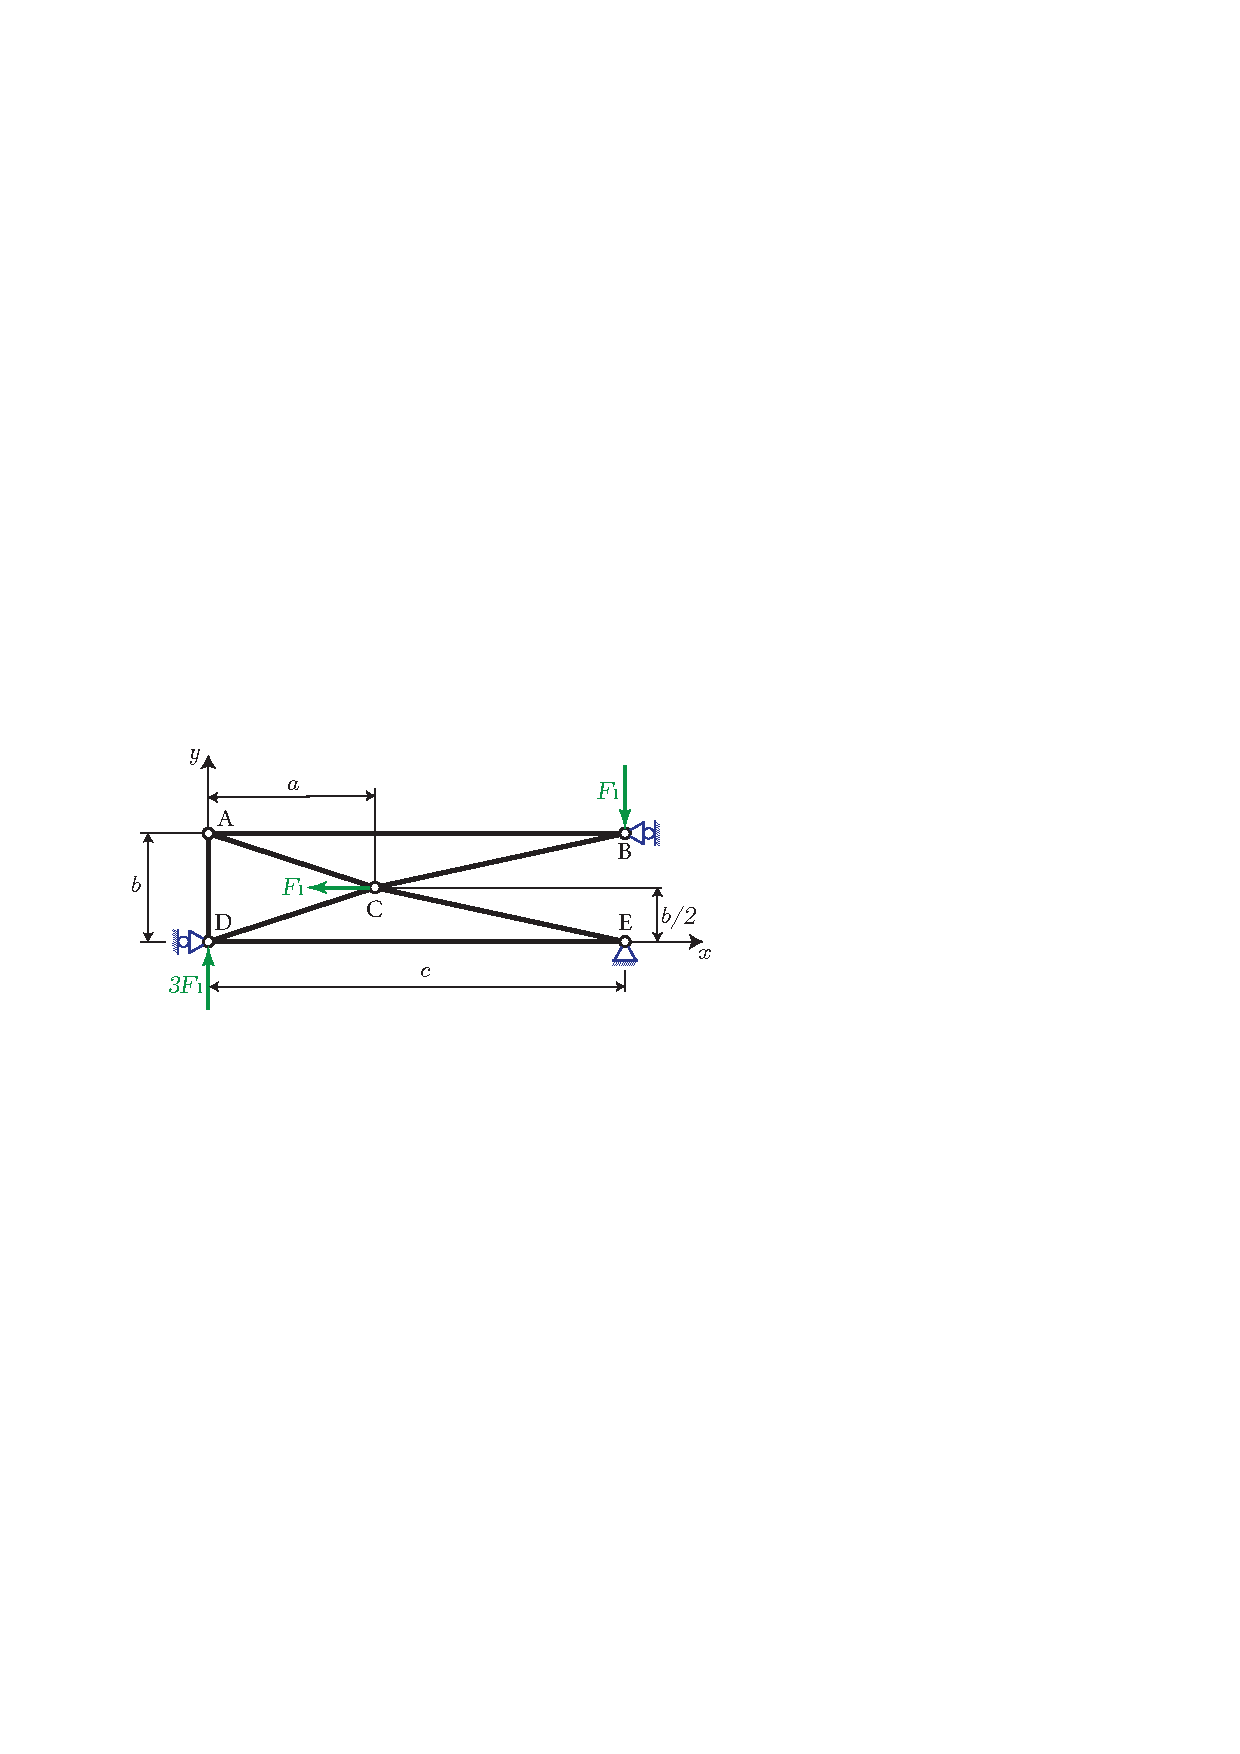
\includegraphics[width=0.85\textwidth]{vszhf1_abra.pdf}
    \caption{A szerkezet léptékhelyes ábrája}
\end{figure}
\subsection{A szerkezet végeselem modelljének ábrája}
Az alábbi ábrán látható a szerkezet VEM modellje:
\begin{figure}[H]
    \centering
    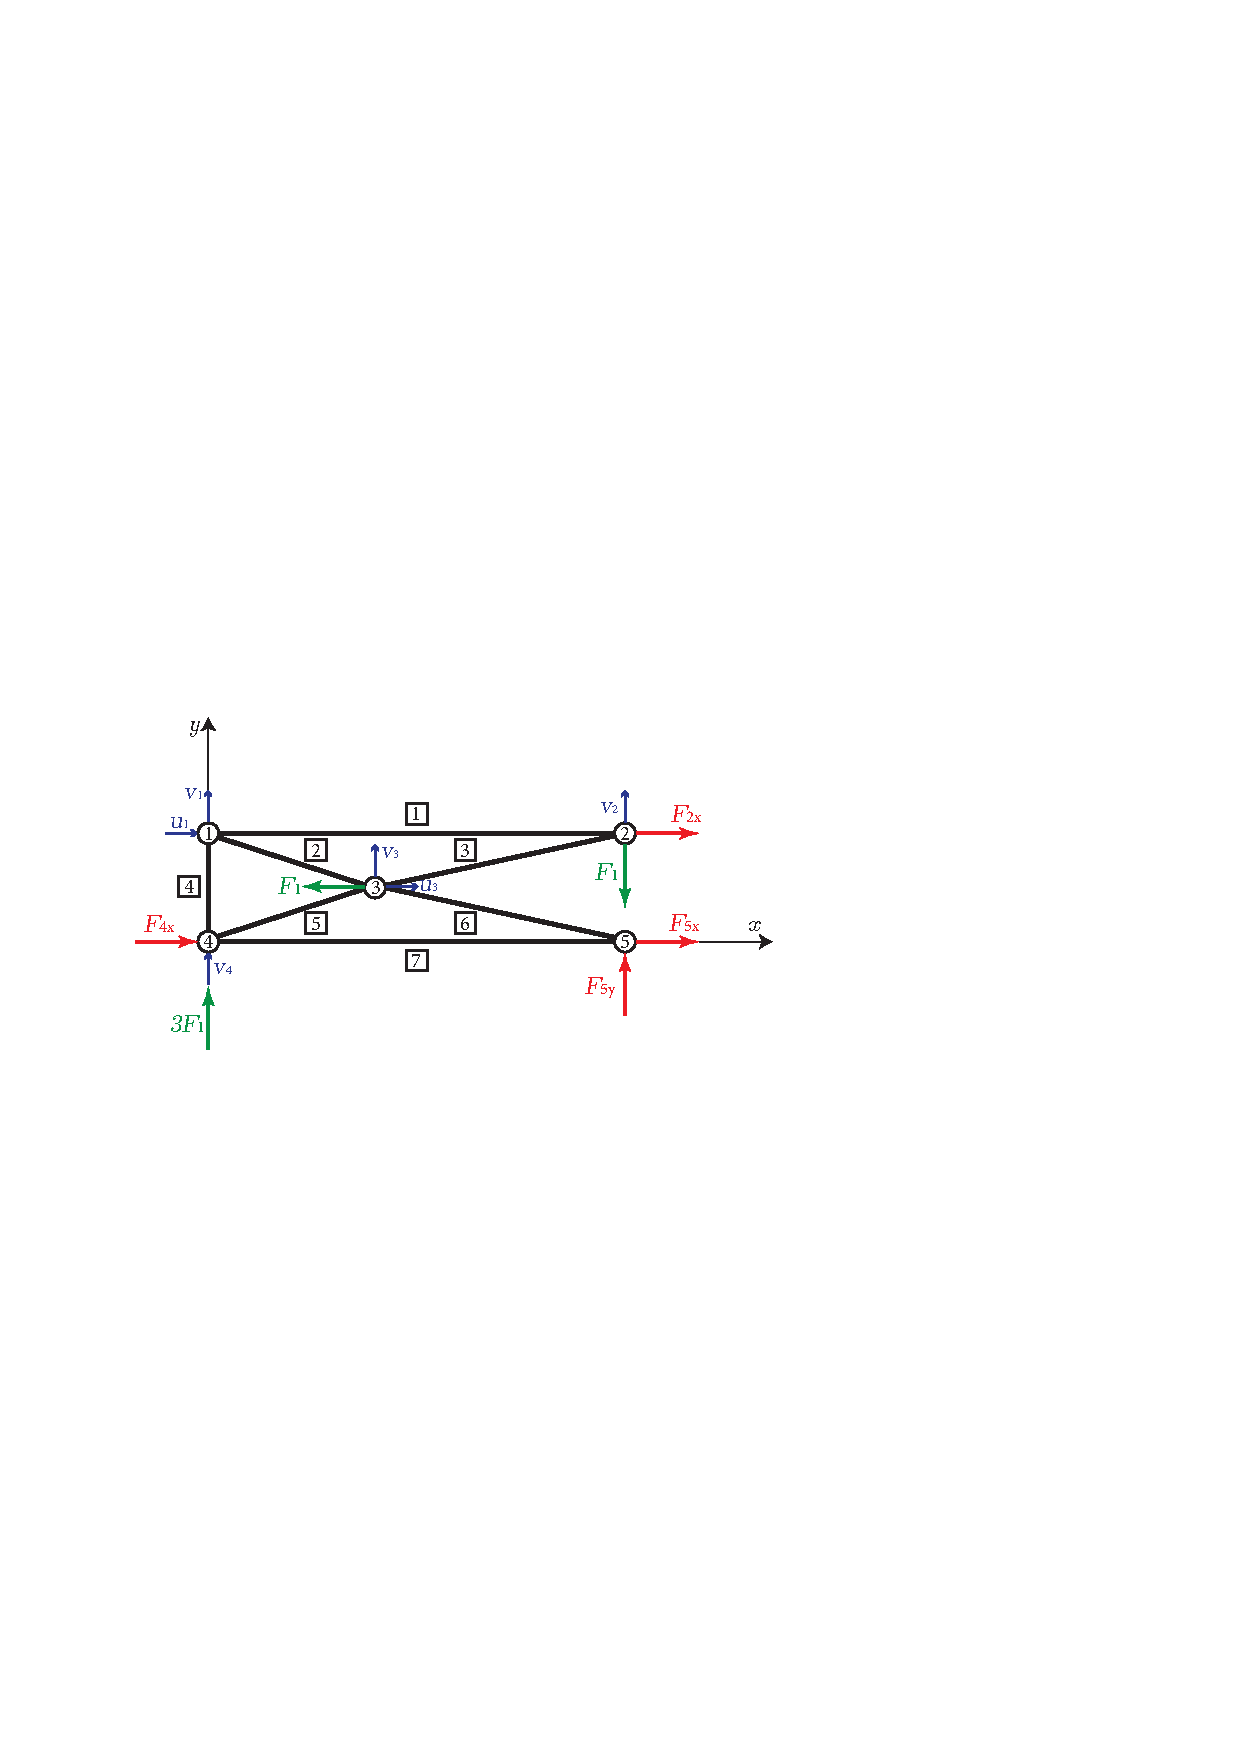
\includegraphics[width=0.85\textwidth]{vszhf1_abra2.pdf}
    \caption{A szerkezet végeselem modelljének felépítése}
\end{figure}
\section{Az elmozduláskomponensek meghatározása}
\subsection{A csomópontok definiálása}
Az alábbi táblázatban láthatóak a különböző csomópontok $x$ illetve
$y$ koordinátái:
\begin{center}
    \begin{tabular}{|c|c|c|}
        \hline
        Csomópont & x koordináta & y koordináta \\
        \hline
        \hline
        1         & 0            & b            \\
        \hline
        2         & c            & b            \\
        \hline
        3         & a            & b/2          \\
        \hline
        4         & 0            & 0            \\
        \hline
        5         & c            & 0            \\
        \hline
    \end{tabular}
\end{center}
\subsection{Elemek hozzárendelése a csomó pontokhoz}
Az alábbi táblázat tartalmazza a csomópont-elem hozzárendeléseket:
\begin{center}
    \begin{tabular}{|c|c|c|}
        \hline
        Elemszám & Lokális első csomópont & Lokális második csomópont \\
        \hline
        \hline
        1        & 1                      & 2                         \\
        \hline
        2        & 1                      & 3                         \\
        \hline
        3        & 2                      & 3                         \\
        \hline
        4        & 1                      & 4                         \\
        \hline
        5        & 3                      & 4                         \\
        \hline
        6        & 3                      & 5                         \\
        \hline
        7        & 4                      & 5                         \\
        \hline
    \end{tabular}
\end{center}
\subsection{Az elemi mennyiségek meghatározása}
\subsubsection{A rúdak hosszainak meghatározása}
A rúdak hosszait az alábbi általános képlet segítségével tudjuk
könnyen kiszámítani:
\begin{equation}
    \boxed{L^{\left(i\right)}=\sqrt{\left(x^{\left(i\right)}_2-x^{\left(i\right)}_1\right)^2+
            \left(y^{\left(i\right)}_2-y^{\left(i\right)}_1\right)^2}}
\end{equation}
Ezen képletet alkalmazva a rúdak hosszai numerikusan az alábbiak:
\begin{multicols}{4}
    \begin{itemize}
        \item $L_1=5 \m$
        \item $L_2=2.1029 \m$
    \end{itemize}
    \columnbreak
    \begin{itemize}
        \item $L_3=3.0696 \m$
        \item $L_4=1.3 \m$
    \end{itemize}
    \columnbreak
    \begin{itemize}
        \item $L_5=2.1029 \m$
        \item $L_6=3.0696 \m$
    \end{itemize}
    \columnbreak
    \begin{itemize}
        \item $L_7=5 \m$
    \end{itemize}
\end{multicols}
\subsubsection{A rúdak szöghelyzeteinek meghatározása}
A rúdak szöghelyzetét legegyszerűbben az alábbi általános összefüggés
segítségével számíthatjuk:
\begin{equation}
    \boxed{\alpha^{\left(i\right)}=
        \arctan \left( \frac{y^{\left(i\right)}_2-y^{\left(i\right)}_1}
        {x^{\left(i\right)}_2-x^{\left(i\right)}_1}\right)}
\end{equation}
Ez alapján a szögek numerikus értékei:
\begin{multicols}{3}
    \begin{itemize}
        \item $\alpha_1=\alpha_7=0 \deg$
        \item $\alpha_2=-18.004 \deg$
    \end{itemize}
    \columnbreak
    \begin{itemize}
        \item $\alpha_3=12.225 \deg$
        \item $\alpha_4=270 \deg$
    \end{itemize}
    \columnbreak
    \begin{itemize}
        \item $\alpha_5=18.004 \deg$
        \item $\alpha_6=-12.225 \deg$
    \end{itemize}
\end{multicols}
\subsubsection{Keresztmetszet jellemzőinek meghatározása}
Keresztmetszetünk esetünkben egy cső amelynek belső átmérője $d$, valamint falvastagsága
$0.15 d$, így ez alapján az alábbi módon számíthatjuk a csőszelvény területét:
\begin{equation}
    A=\frac{\left(\left(1.3 \cdot d\right)^2-d^2\right) \pi }
    {4}=0.00135 \mm
\end{equation}
\subsubsection{Az elemi merevségi mátrixok meghatározása}
Most hogy már ismerjük a rúdak hosszait, szöghelyzeteit valamint Keresztmetszetét,
az alábbi 2D-s húzott-nyomott rúdelemre vonatkozó összefüggéssel meghatározhatjuk a
különböző elemek merevségi mátrixait.
\begin{equation}
    \mx{K}^{\i}=\frac{A \; E}{L^{\i}}
    \begin{bmatrix}
        \cosalfasq          &  & \cosalfa \sinalfa   &  & -\cosalfasq          &  & - \cosalfa  \sinalfa \\
        \cosalfa  \sinalfa  &  & \sinalfasq          &  & - \cosalfa  \sinalfa &  & -\sinalfasq          \\
        -\cosalfasq         &  & -\cosalfa  \sinalfa &  & \cosalfasq           &  & \cosalfa  \sinalfa   \\
        -\cosalfa  \sinalfa &  & -\sinalfasq         &  & \cosalfa  \sinalfa   &  & \sinalfasq           \\
    \end{bmatrix}
\end{equation}
\subsubsection*{Így az elemi merevségi mátrixok:}
\begin{align}
    \mx{K}^{\left(1\right)} & =\mx{K}^{\left(7\right)}=
    \begin{bmatrix}
        5.1482 \futyi  &  & 0 &  & -5.1482 \futyi &  & 0      \\
        0              &  & 0 &  & 0              &  & 0 &  & \\
        -5.1482 \futyi &  & 0 &  & 5.1482 \futyi  &  & 0      \\
        0              &  & 0 &  & 0              &  & 0 &  &
    \end{bmatrix} \Nm                        \\
    \mx{K}^{\left(2\right)} & =
    \begin{bmatrix}
        11.0711 \futyi  &  & -3.5981 \futyi &  & -11.0711 \futyi &  & 3.5981 \futyi  \\
        -3.5981 \futyi  &  & 1.1693 \futyi  &  & 3.5981 \futyi   &  & -1.1693 \futyi \\
        -11.0711 \futyi &  & 3.5981 \futyi  &  & 11.0711 \futyi  &  & -3.5981 \futyi \\
        3.5981 \futyi   &  & -1.1693 \futyi &  & -3.5981 \futyi  &  & 1.1693 \futyi
    \end{bmatrix} \Nm \\
    \mx{K}^{\left(3\right)} & =
    \begin{bmatrix}
        8.0098 \futyi  &  & 1.7354 \futyi  &  & -8.0098 \futyi &  & -1.7354 \futyi \\
        1.7354 \futyi  &  & 0.3760 \futyi  &  & -1.7354 \futyi &  & -0.3760 \futyi \\
        -8.0098 \futyi &  & -1.7354 \futyi &  & 8.0098 \futyi  &  & 1.7354 \futyi  \\
        -1.7354 \futyi &  & -0.3760 \futyi &  & 1.7354 \futyi  &  & 0.3760 \futyi
    \end{bmatrix} \Nm   \\
    \mx{K}^{\left(4\right)} & =
    \begin{bmatrix}
        0 &  & 0               &  & 0 &  & 0              \\
        0 &  & 19.8011 \futyi  &  & 0 &  & -19.801 \futyi \\
        0 &  & 0               &  & 0 &  & 0              \\
        0 &  & -19.8011 \futyi &  & 0 &  & 19.801 \futyi
    \end{bmatrix} \Nm                            \\
    \mx{K}^{\left(5\right)} & =
    \begin{bmatrix}
        11.0711 \futyi  &  & 3.5981 \futyi  &  & -11.0711 \futyi &  & -3.5981 \futyi \\
        3.5981 \futyi   &  & 1.1693 \futyi  &  & -3.5981 \futyi  &  & -1.1693 \futyi \\
        -11.0711 \futyi &  & -3.5981 \futyi &  & 11.0711 \futyi  &  & 3.5981 \futyi  \\
        -3.5981 \futyi  &  & -1.1693 \futyi &  & 3.5981 \futyi   &  & 1.1693 \futyi
    \end{bmatrix} \Nm \\
    \mx{K}^{\left(6\right)} & =
    \begin{bmatrix}
        8.0098 \futyi  &  & -1.7354 \futyi &  & -8.0098 \futyi &  & 1.7354 \futyi  \\
        -1.7354 \futyi &  & 0.3760 \futyi  &  & 1.7354 \futyi  &  & -0.3760 \futyi \\
        -8.0098 \futyi &  & 1.7354 \futyi  &  & 8.0098 \futyi  &  & -1.7354 \futyi \\
        1.7354 \futyi  &  & -0.3760 \futyi &  & -1.7354 \futyi &  & 0.3760 \futyi
    \end{bmatrix} \Nm   \\
\end{align}
\subsubsection{Elemi elmozdulásvektorok meghatározása}
Az elemi elmozdulásvektor alakja minden esetben az alábbi módon néz ki:
\begin{equation}
    \vec{\mathbf{U}}^{\i}=
    \begin{bmatrix}
        {u_1}^{\i} \\
        {v_1}^{\i} \\
        {u_2}^{\i} \\
        {v_2}^{\i}
    \end{bmatrix}
\end{equation}
Ahol:
\begin{itemize}
    \item A felső index az rúdelemre utal
    \item Az alsó indexek pedig a lokális csomópontokra
\end{itemize}
\subsubsection*{Peremfeltételek:}
\begin{itemize}
    \item  Mivel az $\left(1\right)$-es csomópont nincs semmilyen módon
          befogva, így mindkét irányú elmozduláskomponens ébred.
    \item A  $\left(2\right)$-es csomópont görgős csuklóval van rögzítve, így
          csak $y$ irányú elmozduláskomponens ébred. $\; \rightarrow \; \boxed{u_{2}=0 \m}$
    \item A  $\left(3\right)$-as csomópont nincs befogva, így ebben az esetben is mindkét
          irányú elmozduláskomponensünk van.
    \item A $\left(4\right)$-es csomópont is görgős csuklóval van rögzítve
          így csak $y$ irányú elmozduláskomponens ébred. $\; \rightarrow \; \boxed{u_{4}=0 \m}$
    \item Az $\left(5\right)$-ös csomópont csuklóval van befogva, így egyik irányban sem történik
          elmozdulás. $\; \rightarrow \; \boxed{u_{5}=v_{5}=0 \m}$
\end{itemize}
Így az elemi elmozdulásvektorok:
\begin{multicols}{7}
    \noindent
    \begin{equation*}
        \vec{U}^{\left(1\right)}=
        \begin{bmatrix}
            u_1 \\
            v_1 \\
            0   \\
            v_2
        \end{bmatrix}
    \end{equation*}
    \columnbreak
    \begin{equation*}
        \vec{U}^{\left(2\right)}=
        \begin{bmatrix}
            u_1 \\
            v_1 \\
            u_3 \\
            v_3
        \end{bmatrix}
    \end{equation*}
    \columnbreak
    \begin{equation*}
        \vec{U}^{\left(3\right)}=
        \begin{bmatrix}
            0   \\
            v_2 \\
            u_3 \\
            v_3
        \end{bmatrix}
    \end{equation*}
    \columnbreak
    \begin{equation*}
        \vec{U}^{\left(4\right)}=
        \begin{bmatrix}
            u_1 \\
            v_1 \\
            0   \\
            v_4
        \end{bmatrix}
    \end{equation*}
    %\end{multicols}
    %\begin{multicols}{3}
    %    \noindent
    \begin{equation*}
        \vec{U}^{\left(5\right)}=
        \begin{bmatrix}
            u_3 \\
            v_3 \\
            0   \\
            v_4
        \end{bmatrix}
    \end{equation*}
    \columnbreak
    \begin{equation*}
        \vec{U}^{\left(6\right)}=
        \begin{bmatrix}
            u_3 \\
            v_3 \\
            0   \\
            0
        \end{bmatrix}
    \end{equation*}
    \columnbreak
    \begin{equation*}
        \vec{U}^{\left(7\right)}=
        \begin{bmatrix}
            u_4 \\
            v_4 \\
            0   \\
            0
        \end{bmatrix}
    \end{equation*}
\end{multicols}
\subsubsection{Elemi terhelésvektorok meghatározása}
Az elemi terhelésvektor alakja minden esetben az alábbi módon néz ki:
\begin{equation}
    \vec{F}^{\i}=
    \begin{bmatrix}
        F_{1_x}^{\i} \\
        F_{1_y}^{\i} \\
        F_{2_x}^{\i} \\
        F_{2_y}^{\i}
    \end{bmatrix}
\end{equation}
\subsubsection*{Peremfeltételek:}
\begin{itemize}
    \item Mivel az $\left(1\right)$-es csomópont nincs semmilyen módon
          befogva, valamint nem hat rá aktív terhelés, így a benne fellépő
          reakcióerők zérusok. $\; \rightarrow \; \boxed{F_{1_x}=F_{1_y}= 0 \kN}$
    \item A  $\left(2\right)$-es csomópont görgős csuklóval van rögzítve, így
          csak $x$ irányú reakcióerő ébred, valamint az $y$ irányú terhelést már ismerjük.
          $\; \rightarrow \; \boxed{F_{2_y}=-F=-170 \kN}$
    \item A  $\left(3\right)$-as csomópont nincs befogva, valamint egy $x$
          irányú aktív terhelés hat rá, így tehát $\; \rightarrow \; \boxed{F_{3_x}=-F=-170 \kN \hspace{5mm}
                  F_{3_y}=0 \kN}$
    \item A $\left(4\right)$-es csomópont is görgős csuklóval van rögzítve,
          így csak $x$ irányú reakcióerő ébred, valamint az $y$ irányú aktív
          terhelést ismerjük. $\; \rightarrow \; \boxed{F_{4_y}=3 F=510 \kN}$
    \item Az $\left(5\right)$-ös csomópont csuklóval van befogva, így mindkét irányú
          reakcióerő ébred.
\end{itemize}
Így az elemi terhelésvektorok:
\begin{multicols}{7}
    \noindent
    \begin{equation*}
        \vec{F}^{\left(1\right)}=
        \begin{bmatrix}
            0       \\
            0       \\
            F_{2_x} \\
            -F
        \end{bmatrix}
    \end{equation*}
    \columnbreak
    \begin{equation*}
        \vec{F}^{\left(2\right)}=
        \begin{bmatrix}
            0  \\
            0  \\
            -F \\
            0
        \end{bmatrix}
    \end{equation*}
    \columnbreak
    \begin{equation*}
        \vec{F}^{\left(3\right)}=
        \begin{bmatrix}
            F_{2_x} \\
            -F      \\
            -F      \\
            0
        \end{bmatrix}
    \end{equation*}
    \columnbreak
    \begin{equation*}
        \vec{F}^{\left(4\right)}=
        \begin{bmatrix}
            0       \\
            0       \\
            F_{4_x} \\
            3 F
        \end{bmatrix}
    \end{equation*}
    %\end{multicols}
    %\begin{multicols}{3}
    %    \noindent
    \begin{equation*}
        \vec{F}^{\left(5\right)}=
        \begin{bmatrix}
            -F      \\
            0       \\
            F_{4_x} \\
            3 F
        \end{bmatrix}
    \end{equation*}
    \columnbreak
    \begin{equation*}
        \vec{F}^{\left(6\right)}=
        \begin{bmatrix}
            -F      \\
            0       \\
            F_{5_x} \\
            F_{5_y}
        \end{bmatrix}
    \end{equation*}
    \columnbreak
    \begin{equation*}
        \vec{F}^{\left(7\right)}=
        \begin{bmatrix}
            F_{4_x} \\
            3 F     \\
            F_{5_x} \\
            F_{5_y}
        \end{bmatrix}
    \end{equation*}
\end{multicols}
\subsection{Globális mennyiségek meghatározása}
\subsubsection{Globális merevségi mátrix meghatározása}
Esetünkben öt csomópontunk van, valamint mindegyik 2-2 szabadságfokkal rendelkezik,
így összesen 10 szabadsági fokunk van.
Rendeljünk hozzá a szabadságfokokat mindegyik rúdelemünkhöz, az alábbi mátrixba rendezve:
\begin{equation}
    \mx{DoF}=
    \begin{blockarray}{ccccc}
        {u_1}^{\i} & {v_1}^{\i} & {u_2}^{\i} & {v_2}^{\i} \\
        \begin{block}{[cccc]c}
            1 & 2 & 3 & 4 & \left(\mathbf{1}\right) \\
            1 & 2 & 5 & 6 & \left(\mathbf{2}\right) \\
            3 & 4 & 5 & 6 & \left(\mathbf{3}\right) \\
            1 & 2 & 7 & 8 & \left(\mathbf{4}\right) \\
            5 & 6 & 7 & 8 & \left(\mathbf{5}\right) \\
            5 & 6 & 9 & 10 & \left(\mathbf{6}\right) \\
            7 & 8 & 9 & 10 & \left(\mathbf{7}\right) \\
        \end{block}
    \end{blockarray}
\end{equation}
A globális merevségi mátrixot úgy kell elő állítanunk, hogy
az adott elemhez tartozó merevségi mátrix elemeit a megfelelő szabadsági
fokhoz tartozó helyhez rendeljük hozzá. Ezután az alábbi numerikus eredményt kapjuk:
{\tiny
\begin{equation}
    \mx{K}=
    \begin{bmatrix}
        16.2194  & -3.5981  & -5.1483 & 0       & -11.0711 & 3.5981  & 0        & 0        & 0       & 0       \\
        -3.5981  & 20.9705  & 0       & 0       & 3.5981   & -1.1694 & 0        & -19.8011 & 0       & 0       \\
        -5.1483  & 0        & 13.1582 & 1.7355  & -8.0099  & -1.7355 & 0        & 0        & 0       & 0       \\
        0        & 0        & 1.7355  & 0.3760  & -1.7355  & -0.3760 & 0        & 0        & 0       & 0       \\
        -11.0711 & 3.5981   & -8.0099 & -1.7355 & 38.1620  & 0       & -11.0711 & -3.5981  & -8.0099 & 1.7355  \\
        3.5981   & -1.1694  & -1.7355 & -0.3760 & 0        & 3.0908  & -3.5981  & -1.1694  & 1.7355  & -0.3760 \\
        0        & 0        & 0       & 0       & -11.0711 & -3.5981 & 16.2194  & 3.5981   & -5.1483 & 0       \\
        0        & -19.8011 & 0       & 0       & -3.5981  & -1.1694 & 3.5981   & 20.9705  & 0       & 0       \\
        0        & 0        & 0       & 0       & -8.0099  & 1.7355  & -5.1483  & 0        & 13.1582 & -1.7355 \\
        0        & 0        & 0       & 0       & 1.7355   & -0.3760 & 0        & 0        & -1.7355 & 0.3760  \\
    \end{bmatrix} \futyi \Nm
\end{equation}}
\subsubsection{Globális elmozdulásvektor meghatározása}
A globális elmozdulásvektor az alábbi módon nézn ki, a peremfeltételeket
figyelembe véve:
\noindent
\begin{equation}
    \vec{\mathbf{U}}=
    \begin{bmatrix}
        u_1 &
        v_1 &
        0   &
        v_2 &
        u_3 &
        v_3 &
        0   &
        v_4 &
        0   &
        0
    \end{bmatrix}^{T}
\end{equation}
\subsubsection{Globális terhelésvektor meghatározása}
A globális terhelésvektor az alábbi módon nézn ki, a peremfeltételeket
figyelembe véve:
\begin{equation}
    \vec{\mathbf{F}}=
    \begin{bmatrix}
        0       &
        0       &
        F_{2_x} &
        -F      &
        -F      &
        0       &
        F_{4_x} &
        3 F     &
        F_{5_x} &
        F_{5_y}
    \end{bmatrix}^{T}
\end{equation}
\subsection{Az elmozduláskomponensek kiszámítása}
Ahhoz hogy megtudjuk határozni a csomópontok elmozduláskomponenseit az alábbi
egyenletrendszert kell megoldanunk:
\begin{equation}
    \boxed{
        \vec{U}=\mx{K}^{-1} \vec{F}}
\end{equation}
\subsubsection{Az egyenletrendszer kondenzálása}
Ezt az egyenletrendszert azonban nem tudjuk megoldani, hiszen $\mx{\vec{F}}$
vektorban is vannak ismeretlen elemek, így egyenlet kondenzációt kell végeznünk,
ami azt jelenti hogy a zérus elmozduláshoz tartozó sorokat és oszlopokat nem vesszük figyelembe
a kondenzált egyenletrendszer felírásakor. Így a felírt
kondenzált egyenletrendszer:
{\tiny
\begin{equation}
    \underbrace{
    \begin{bmatrix}
        1.6219 \cdot 10^{8}  & -3.5981 \cdot 10^{7} & 0                    & -1.1071 \cdot 10^{8} & 3.5981 \cdot 10^{7}  & 0                    \\
        -3.5981 \cdot 10^{7} & 2.0970 \cdot 10^{8}  & 0                    & 3.5981 \cdot 10^{7}  & -1.1694 \cdot 10^{7} & -1.9801 \cdot 10^{8} \\
        0                    & 0                    & 3.7602 \cdot 10^{6}  & -1.7355 \cdot 10^{7} & -3.7602 \cdot 10^{6} & 0                    \\
        -1.1071 \cdot 10^{8} & 3.5981 \cdot 10^{7}  & -1.7355\cdot 10^{7}  & 3.8162 \cdot 10^{8}  & 0                    & -3.5981 \cdot 10^{7} \\
        3.5981 \cdot 10^{7}  & -1.1694 \cdot 10^{7} & -3.7602 \cdot 10^{6} & 0                    & 3.0908 \cdot 10^{7}  & -1.1694 \cdot 10^{7} \\
        0                    & -1.9801 \cdot 10^{8} & 0                    & -3.5981 \cdot 10^{7} & -1.1694 \cdot 10^{7} & 2.0970 \cdot 10^{8}
    \end{bmatrix}^{-1}}_{\vec{\hat{K}}^{-1}}
    \underbrace{\begin{bmatrix}
            0       \\
            0       \\
            -170000 \\
            -170000 \\
            0       \\
            510000  \\
        \end{bmatrix}}_{\vec{\hat{F}}}=
    \underbrace{\begin{bmatrix}
            0.0212 \\
            0.2071 \\
            0.1714 \\
            0.0136 \\
            0.1532 \\
            0.2088
        \end{bmatrix}}_{\vec{\hat{U}}} \m
\end{equation}}
\subsubsection*{A csomóponti elmozdulások tehát:}
\begin{multicols}{2}
    \begin{itemize}
        \item $u_1=21.2094 \mili$
        \item $v_1=207.0613 \mili$
        \item $v_2=171.4109 \mili$
    \end{itemize}
    \columnbreak
    \begin{itemize}
        \item $u_3=13.6717 \mili$
        \item $v_3=153.5211 \mili$
        \item $v_4=208.8535 \mili$
    \end{itemize}
\end{multicols}
\subsubsection{A globális elmozdulásvektor numerikus értékei}
Az $\vec{\hat{U}}$ vektor és a peremfeltételek segítségével fel tudjuk írni már
a globális elmozdulásvektort.
\begin{equation}
    \vec{U}=
    \begin{bmatrix}
        21.2094  &
        207.0613 &
        0        &
        171.4109 &
        13.6717  &
        153.5211 &
        0        &
        208.8535 &
        0        &
        0
    \end{bmatrix}^{T} \mili
\end{equation}
\newpage
\section{A deformált alak ábrázolása}
A szerkezet deformált alakja az alábbi módon néz ki az elmozduláskomponensek xy-szoros
nagyítása esetén:
\begin{figure}[H]
    \centering
    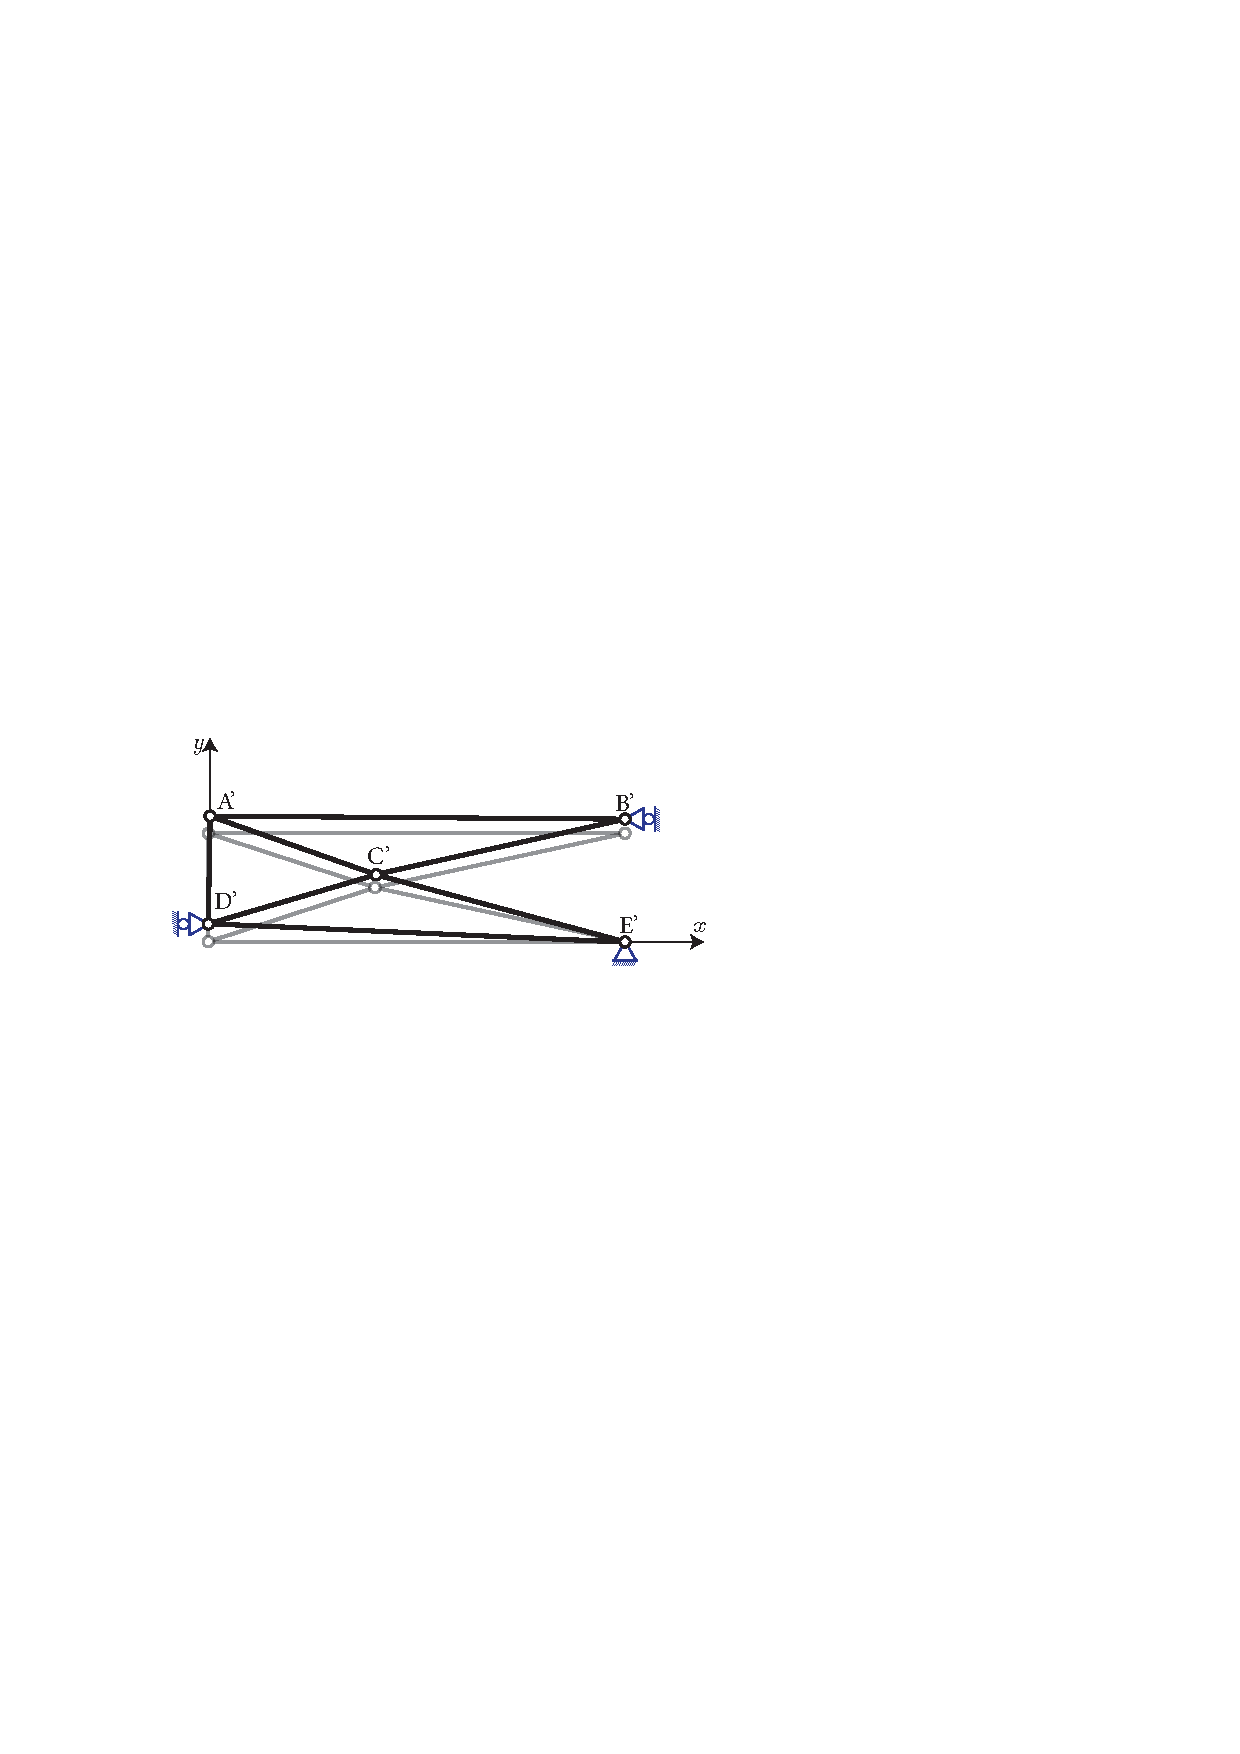
\includegraphics[width=0.8\textwidth]{vszhf1_def.pdf}
    \caption{A deformált szerkezet ábrája}
\end{figure}
\section{A reakcióerők meghatározása}
\subsection{Globális terhelésvektor kiszámítása}
Ahhoz, hogy kiszámítsuk a globális terhelésvektort csak bekell helyettesítenünk
az alábbi kondenzálatlan egyenletrendszerbe:
\begin{equation}
    \vec{F}=\mx{K} \; \vec{U}=
    \begin{bmatrix}
        0        \\
        0        \\
        -1876.53 \\
        -170     \\
        -170     \\
        0        \\
        477.31   \\
        510      \\
        1569.23  \\
        -340
    \end{bmatrix} \kN
\end{equation}
\subsection{A reakcióerő vektor kiszámítása}
A reakcióerő vektort úgy tudjuk kiszámolni, hogy kivonjuk a globális
terhelésvektorból az aktív terhelések vektorát.
\begin{equation}
    \vec{F_r}=\vec{F}-\vec{F_a}=
    \begin{bmatrix}
        0        \\
        0        \\
        -1876.53 \\
        -170     \\
        -170     \\
        0        \\
        477.31   \\
        510      \\
        1569.23  \\
        -340
    \end{bmatrix}-
    \begin{bmatrix}
        0    \\
        0    \\
        0    \\
        -170 \\
        -170 \\
        0    \\
        0    \\
        510  \\
        0    \\
        0
    \end{bmatrix}=
    \begin{bmatrix}
        0        \\
        0        \\
        -1876.53 \\
        0        \\
        0        \\
        0        \\
        477.31   \\
        0        \\
        1569.23  \\
        -340
    \end{bmatrix} \kN
\end{equation}
\subsubsection*{Tehát a reakcióerők:}
\begin{multicols}{2}
    \begin{itemize}
        \item $F_{2_x}= -1876.53 \kN$
        \item $F_{4_x}=477.31 \kN$
    \end{itemize}
    \columnbreak
    \begin{itemize}
        \item $F_{5_x}= 1569.23 \kN$
        \item $F_{5_y}= -340 \kN$
    \end{itemize}
\end{multicols}
\section{A rudak normálfeszültségeinek meghatározása}
\subsection{A rudak megnyúlásának kiszámítása}
Ahhoz meg tudjuk határozni a rudakban ébredő normálfeszültségeket,
célszerű először a rudak megnyúlását kiszámítani, amit az alábbi összefüggés
segítségével tehetünk meg:
\begin{equation}
    \boxed{
    \varepsilon^{\i}=\frac{(u_2^{\i}-u_1^{\i})
    \cos \left(\alpha^{\i}\right)+(v_2^{\i}-v_1^{\i})
    \sin \left(\alpha^{\i}\right)}{L^{\i}}
    }
\end{equation}
\subsubsection*{Tehát a rudak megnyúlásái numerikusan:}
\begin{multicols}{2}
    \begin{itemize}
        \item $\varepsilon_1= -0.00424 \fos$
        \item $\varepsilon_2= 0.00446 \fos$
        \item $\varepsilon_3= -0.00311 \fos$
        \item $\varepsilon_4= -0.00137 \fos$
    \end{itemize}
    \columnbreak
    \begin{itemize}
        \item $\varepsilon_5= -0.00194  \fos$
        \item $\varepsilon_6=  0.00623 \fos$
        \item $\varepsilon_7=  0 \fos$
    \end{itemize}
\end{multicols}
\subsection{A rudak normálfeszültségeinek kiszámítása}
Most pedig a már jól ismert Hooke-törvény segítségével számíthatjuk ki
a kívánt mennyiségeket.
\begin{equation}
    \boxed{\sigma^{\i}=E \cdot \varepsilon^{\i}}
\end{equation}
\subsubsection*{Tehát a rudakban ébredő normálfeszültségek értékei:}
\begin{multicols}{2}
    \begin{itemize}
        \item $\sigma_1= -805.95212 \Mpa$
        \item $\sigma_2=  847.455 \Mpa$
        \item $\sigma_3=  -592.567 \Mpa$
        \item $\sigma_4=  -261.937 \Mpa$
    \end{itemize}
    \columnbreak
    \begin{itemize}
        \item $\sigma_5= -370.445 \Mpa$
        \item $\sigma_6=  1185.139 \Mpa$
        \item $\sigma_7=  0 \Mpa$
    \end{itemize}
\end{multicols}
\newpage
\tableofcontents

\subsection*{Felhasznált szoftverek:}
\begin{itemize}
    \item \LaTeX \hspace{0.4mm} szövegszerkesztő: VS Code
    \item Ábrák rajzolása: Adobe Illustrator
    \item Számítások elvégzése: JuPyter Notebook
    \item Számítások ellenőrzése: SIKER 2009
\end{itemize}


\end{document}